\documentclass[10pt]{article}
\usepackage[margin=0.7in]{geometry}
\usepackage{amsmath}
\usepackage{amssymb}
\usepackage{amsfonts}
\usepackage{hyperref}
\usepackage{enumitem}
\usepackage{enotez}
\usepackage{tikz}
\usepackage{pgfplots}
\usetikzlibrary{matrix, arrows.meta, positioning}
\hypersetup{colorlinks=true, urlcolor=blue}
\DeclareMathOperator*{\argmax}{argmax}


\begin{document}

\title{Spectral Derivatives}
\author{Pavel Komarov}
\date{January 8, 2025}
\maketitle

One of the happiest accidents in all math is the ease of taking derivatives in the Fourier (i.e. the \textit{frequency}) domain. But in order to exploit this extraordinary fact without serious artefacting, and in order to be able to use a computer, we need quite a bit of extra knowledge and care.

This document sets out the math behind the \texttt{spectral-derivatives} package, all the way down to the bones, as much as I can manage. I try to get in to the real \textit{whys} behind what we're doing here, touching on fundamental signal processing and calculus concepts as necessary, and building upwards to more general cases.

% Add an enumerate here to outline things? Or a table of contents?

\section{Bases}

A \textit{basis} is a set of ``orthogonal" functions, call them $\{\xi_k\}$, that can be summed together in various quantities to produce other functions. Othogonal means that if we take the ``inner product" of one funtion from the set with itself, we get back 1, and if we take the inner product of a function with a different memnber of the set, we get back 0. In this sense the members of the basis set are independent of one another, just like perpendicular directions on a graph.

The inner product between two functions $f$ and $g$ is a generalization of the inner product between vectors, where instead of summing over a finite number of discrete entries, we integrate over infinitely many infinitesimally-separated points in the domain. We define it as:

$$ \langle f,g \rangle = \int\limits_{-\infty}^{\infty} \overline{f(x)} g(x) dx $$

where the overbar $\overline{\cdot}$ denotes a complex conjugate.\newline

The inner product is symmetrical, so

$$ \langle f,g \rangle = \langle g,f \rangle = \int\limits_{-\infty}^{\infty} f(x) \overline{g(x)} dx $$

Notice that this integral could diverge. If it doesn't, we say the argument is \href{https://mathworld.wolfram.com/LebesgueIntegrable.html}{``Lebesgue integrable"}\cite{lebesgue}. Much of what we'll do only makes sense for this class of functions, so be aware.

\subsection{The Fourier Basis}

The most famous basis is the \textit{Fourier} basis\endnote{There's a great passage in Richard Hamming's book \textit{The Art of Doing Science and Engineering}\cite{hamming} where he wonders why we use the Fourier basis so much:

\begin{quotation}
``It soon became clear to me digital filter theory was dominated by Fourier series, about which theoretically I had learned in college, and actually I had had a lot of further education during the signal processing I had done for John Tukey, who was a professor from Princeton, a genius, and a one or two day a week employee of Bell Telephone Laboratories. For about ten years I was his computing arm much of the time.

Being a mathematician I knew, as all of you do, that any complete set of functions will do about as good as any other set at representing arbitrary functions. Why, then, the exclusive use of the Fourier series? I asked various electrical engineers and got no satisfactory answers. One engineer said alternating currents were sinusoidal, hence we used sinusoids, to which I replied it made no sense to me. So much for the usual residual education of the typical electrical engineer after they have left school!

So I had to think of basics, just as I told you I had done when using an error-detecting computer. What is really going on? I suppose many of you know what we want is a time-invariant representation of signals, since there is usually no natural origin of time. Hence we are led to the trigonometric functions (the eigenfunctions of translation), in the form of both Fourier series and Fourier integrals, as the tool for representing things.

Second, linear systems, which is what we want at this stage, also have the same eigenfunctions—the complex exponentials which are equivalent to the real trigonometric functions. Hence a simple rule: if you have either a time-invariant system or a linear system, then you should use the complex exponentials.

On further digging into the matter I found yet a third reason for using them in the field of digital filters. There is a theorem, often called Nyquist's sampling theorem (though it was known long before and even published by Whittaker, in a form you can hardly realize what it is saying, even when you know Nyquist's theorem), which says that if you have a band-limited signal and sample at equal spaces at a rate of at least two in the highest frequency, then the original signal can be reconstructed from the samples. Hence the sampling process loses no information when we replace the continuous signal with the equally spaced samples, provided the samples cover the whole real line. The sampling rate is often known as the Nyquist rate after Harry Nyquist, also of servo stability fame, as well as other things [also reputed to have been just a really great guy who often had productive lunches with his colleagues, giving them feedback and asking questions that brought out the best in them]. If you sample a non-band-limited function, then the higher frequencies are ``aliased" into lower ones, a word devised by Tukey to describe the fact that a single high frequency will appear later as a single low frequency in the Nyquist band. The same is not true for any other set of functions, say powers of $t$. Under equally spaced sampling and reconstruction a single high power of t will go into a polynomial (many terms) of lower powers of $t$.

Thus there are three good reasons for the Fourier functions: (1) time invariance, (2) linearity, and (3) the reconstruction of the original function from the equally spaced samples is simple and easy to understand.

Therefore we are going to analyze the signals in terms of the Fourier functions, and I need not discuss with electrical engineers why we usually use the complex exponents as the frequencies instead of the real trigonometric functions. [It's down to convenience, really.] We have a linear operation, and when we put a signal (a stream of numbers) into the filter, then out comes another stream of numbers. It is natural, if not from your linear algebra course then from other things such as a course in differential equations, to ask what functions go in and come out exactly the same except for scale. Well, as noted above, they are the complex exponentials; they are the eigenfunctions of linear, time-invariant, equally spaced sampled systems.

Lo and behold, the famous transfer function [contains] exactly the eigenvalues of the corresponding eigenfunctions! Upon asking various electrical engineers what the transfer function was, no one has ever told me that! Yes, when pointed out to them that it is the same idea they have to agree, but the fact it is the same idea never seemed to have crossed their minds! The same, simple idea, in two or more different disguises in their minds, and they knew of no connection between them! Get down to the basics every time!"\end{quotation}}, which is the set of complex exponentials

\begin{equation}\label{euler}
e^{j \omega} = \cos(\omega) + j \sin(\omega)
\end{equation}

where I'm using $j$ to represent the imaginary unit, because I'm from Electrical Engineering, and because Python uses \texttt{j}.\newline

Why this identity is true isn't obvious at first but can be seen by \href{https://math.stackexchange.com/a/492165/278341}{Taylor Expanding}\cite{taylor} the exponential function and trigonometric functions:

$$e^x = 1 + x + \frac{x^2}{2!} + \frac{x^3}{3!} + ... = \sum_{n=0}^{\infty} \frac{x^n}{n!}$$

So

$$ e^{j \omega} = 1 + j \omega + \frac{(j \omega)^2}{2!} + \frac{(j \omega)^3}{3!} + ... = 1 + j \omega - \frac{\omega^2}{2!} - j \frac{\omega^3}{3!} + \frac{\omega^4}{4!} - ... $$

$$ \sin(\omega) = \omega - \frac{\omega^3}{3!} + \frac{\omega^5}{5!} - \frac{\omega^7}{7!} + ... $$

$$ \cos(\omega) = 1 - \frac{\omega^2}{2!} + \frac{\omega^4}{4!} - \frac{\omega^6}{6!} + ... $$

Notice all of the even-power terms appear with alternating sign as in the cosine expansion, and the odd-power terms appear with alternating sign as in the sine expansion, but with an extra $j$ multiplied in.

The presence of complex numbers to make this work can be confusing at first, but don't be scared! All we're really doing is using a compressed representation of a sine plus a cosine, where the real and imaginary parts (orthogonal in the complex plane, and therefore independent and non-interfering) allow us to describe the contributions of sine and cosine simultaniously. In fact, \href{https://math.stackexchange.com/a/1293127/278341}{Joseph Fourier originally used only real trigonometric functions}\cite{complex}, and it wasn't until later someone decided it would be easier to work with complex exponentials. Later (\autoref{fourier}) we'll see that for real signals all the complex numbers cancel, leaving only a \textit{real} sine and \textit{real} cosine, which when added together make \textit{a single, phase-shifted sinusoid!} So think of $e^{j \omega}$ as oscillations at a particular frequency, $\omega$.

If we inner product mismatched wiggles, they misalign and integrate to 0, but if we inner product matched wiggles, they align, multiply to 1 because of the complex conjugate, and integrate to $2\pi$ over a period.

\section{Transforms}

I can use a basis to ``transform" a function, meaning I take the function's inner product with each of the basis functions to produce numbers:

$$ \langle f,\xi_k \rangle = \int\limits_{-\infty}^{\infty} f(x) \overline{\xi_k(x)} dx = \text{a constant coefficient}, c_k $$

These numbers descibe \textit{how much} of each basis function $\xi_k$ is present in the signal $f$. If I do this for all the $\{\xi_k\}$, I essentially get a \textit{recipe}, which says ``I need this much of $\xi_0$ and that much of $\xi_1$ and howevermuch of $\xi_2$ ... added together to reproduce the original signal."

$$ f(x) = \sum_{k=0}^{M-1} c_k \xi_k(x) $$

where $M$ is the number of basis functions I'm using in my reconstruction.\newline

The set of numbers $c_k$ is now \textit{an alternative representation} of the original function. In some sense it's equally descriptive, so long as we know which basis we're using to reconstruct. We've \textit{transformed} to a different domain.

Beware that the terminology ``transform" and ``domain" is not always used to describe transforming a continuous function to a discrete series like this. However, it is possible the basis set has infinitely many members which are in some sense dense, infinitesimally close together. This is indeed the case for the Fourier basis, where we choose $\omega \in \mathbb{R}$, and hence $\omega$ really can become a new domain. (For the relationship between different variants of the Fourier transform, see \autoref{family}.) 

\subsection{The Fourier Transform}\label{fourier}

Using Fourier's original sinusoid formulation, we can write the reconstruction expression as:

$$ f(x) = a_0 + \sum_{k=1}^{\infty} (a_k \cos(k \omega_0 x) + b_k \sin(k \omega_0 x))$$

where
\begin{itemize}[noitemsep, topsep=0pt, after=\newline]
	\item $a_k$ and $b_k$ are coefficients describing how much cosine and sine to add in, respectively
	\item $\omega_0$ is a fundamental frequency, so the $k^{th}$ frequency becomes $k \cdot \omega_0$
\end{itemize}

Let's now use $\cos(x) = \frac{e^{jx} + e^{-jx}}{2}$ and $\sin(x) = \frac{e^{jx} - e^{-jx}}{2j}$, which can be verified by manipulating Euler's formula, \autoref{euler}.

\begin{align*}
f(x) &= a_0 + \sum_{k=1}^{\infty} (a_k \frac{e^{j k \omega_0 x} + e^{-j k \omega_0 x}}{2} + b_k \frac{e^{j k \omega_0 x} - e^{-j k \omega_0 x}}{2j}) \\
&= a_0 + \sum_{k = -\infty}^{-1} (\frac{a_{-k}}{2} - \frac{b_{-k}}{2j}) e^{j k \omega_0 x} + \sum_{k = 1}^{\infty} (\frac{a_k}{2} + \frac{b_k}{2j}) e^{j k \omega_0 x} = \sum_{k = -\infty}^{\infty} c_k e^{j k \omega_0 x}
\end{align*}

So if we choose $c_0 = a_0$ and $c_k = \overline{c_{-k}} = \frac{a_k}{2} + \frac{b_k}{2j}$, then the complex exponential formulation is \href{http://lpsa.swarthmore.edu/Fourier/Series/DerFS.html}{exactly equivalent to the trigonometric formulation}\cite{swarthmore}. That is, we can choose \textit{complex} $c_k$ such that when multiplied by \textit{complex} exponentials, we get back only \textit{real} signal! Essentially, the relative balance of real and complex in $c_k$ affects how much cosine and sine are present at the $k^{th}$ frequency, thereby accomplishing a phase shift. Without accounting for phase shifts, we would only be able to model \textit{symmetric} signals!

If instead of a fundamental frequency $\omega_0 = \frac{2\pi}{T}$, where $T$ is a period of repetition, the signal contains dense frequencies (because it has no repetition, $T \rightarrow \infty$, $\omega_0 \rightarrow 0$), then it makes more sense to express the transformed coefficients as a function in $\omega$ and to make both our inner product and reconstruction expression integrals:


\begin{equation}\label{pair}
\begin{aligned}
\hat{f}(\omega) &= \int\limits_{-\infty}^{\infty} f(x) e^{-j \omega x} dx = \mathcal{F}\{f(x)\} \\
f(x) &= \frac{1}{2\pi} \int\limits_{-\infty}^{\infty} \hat{f}(\omega) e^{j \omega x} d \omega = \mathcal{F}^{-1}\{\hat{f}(\omega)\}
\end{aligned}
\end{equation}


where the hat $\hat{\cdot}$ represents a function in the Fourier domain, and the $\frac{1}{2\pi}$ is a scaling factor that corrects for the fact the inner product of a Fourier basis function with itself integrates to $2\pi$ over a period instead of to $1$ as we need for orthonormality.

Just like the $c_k$, $\hat{f}(\omega)$ can be complex, but if the original $f(x)$ is real, then $\hat{f}$'s complexity will perfectly interact with the complex exponentials to produce only a real function in the reconstruction. 

\subsection{A Whole Family}\label{family}

Part of what makes Fourier transforms confusing is the proliferation of different variants for different situations, so it's worth \href{https://medium.com/sho-jp/fourier-transform-101-part-4-discrete-fourier-transform-8fc3fbb763f3 }{categorizing them}.\cite{medium}. First off, are we dealing with a periodic signal (which has an $\omega_0$) or an aperiodic signal (which doesn't)? And second, are we dealing with a continuous function or discrete samples?

\begin{center}
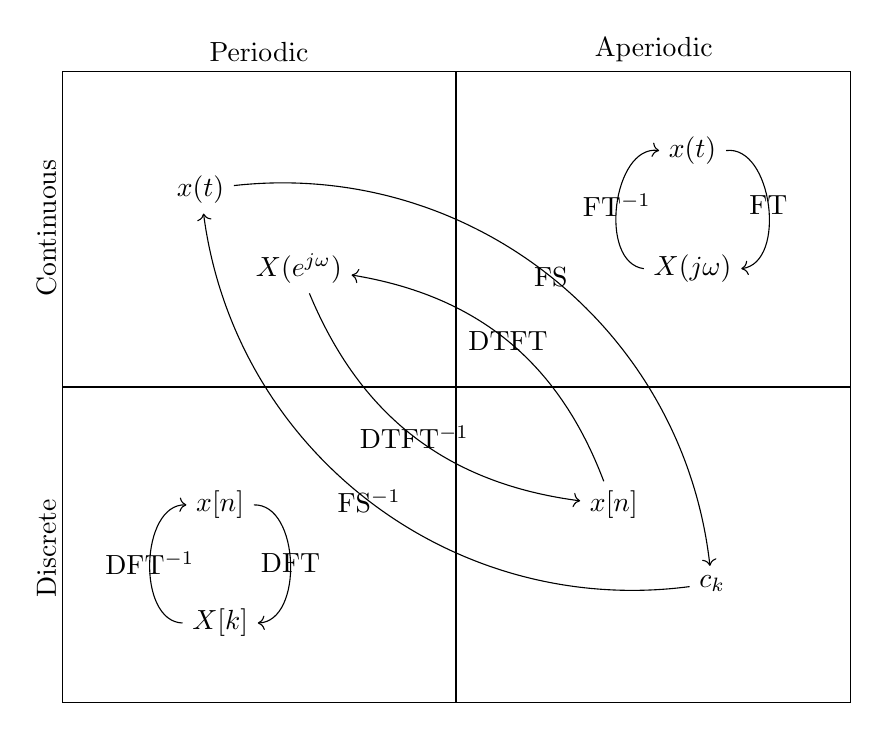
\begin{tikzpicture}
\matrix (m) [
  matrix of nodes,
  nodes={draw, align=center, text height=1.5ex, text depth=.25ex, anchor=center}, column sep=0pt, row sep=0pt,
  cells={nodes={draw, minimum width=5cm, minimum height=4cm, outer sep=0pt}}
] at (0, 0) {
  \node (A) {}; & \node (B) {}; \\
  \node (C) {}; & \node (D) {}; \\
};

\node[anchor=south] at (A.north) {Periodic};
\node[anchor=south] at (B.north) {Aperiodic};
\node[anchor=east, rotate=90, yshift=2mm, xshift=10mm] at (A.west) {Continuous};
\node[anchor=east, rotate=90, yshift=2mm, xshift=7mm] at (C.west) {Discrete};

\node at (-3.25,2.5) (x_t_periodic) {$x(t)$}; 
\node at (-2,1.5) (X_ejw) {$X(e^{j\omega}$)};
\node at (3,3) (x_t_aperiodic) {$x(t)$}; 
\node at (3,1.5) (X_jw) {$X(j\omega$)};
\node at (-3, -1.5) (x_n_periodic) {$x[n]$};
\node at (-3, -3) (X_k) {$X[k]$};
\node at (2, -1.5) (x_n_aperiodic) {$x[n]$};
\node at (3.25, -2.5) (c_k) {$c_k$};

\draw[->, bend right=30] (X_ejw) to node[midway] {DTFT$^{-1}$} (x_n_aperiodic);
\draw[->, bend right=30] (x_n_aperiodic) to node[midway] {DTFT} (X_ejw);
\draw[->, bend left=45] (c_k) to node[midway] {FS$^{-1}$} (x_t_periodic);
\draw[->, bend left=45] (x_t_periodic) to node[midway] {FS} (c_k);
\draw[->, bend left=90] (X_k) to node[midway] {DFT$^{-1}$} (x_n_periodic);
\draw[->, bend left=90] (x_n_periodic) to node[midway] {DFT} (X_k);
\draw[->, bend left=90] (x_t_aperiodic) to node[midway] {FT} (X_jw);
\draw[->, bend left=90] (X_jw) to node[midway] {FT$^{-1}$} (x_t_aperiodic);
\end{tikzpicture}
\end{center}

Here FS stands for ``Fourier Series", which is the first situation covered above. FT stands for ``Fourier Transform", which is given by the integral pair, \autoref{pair}. But these are not the only possibilities! DTFT stands for ``Discrete Time Fourier Transform", where the signal we want to analyze is discrete but the transform is continuous. And finally DFT stands for ``Discrete Fourier Transform", not to be confused with the DTFT, which we use when \textit{both} the original and transformed signals are sampled.

\textit{All} of these can be considered Fourier transforms, but often when people talk about \textit{the} canonical ``Fourier Transform", they are referring to the continuous, aperiodic case in the upper righthand cell.

The notation of all these different functions and transforms is easy to mix up and made all the more confusing by the reuse of symbols. But it's important to keep straight which situation we're in. I can only apologize. For more on all these, see \cite{oppenheim}.

\section{Taking Derivatives in the Fourier Domain}

Let's \href{https://www.youtube.com/watch?v=d5d0ORQHNYs}{take a Fourier transform of the derivative of a function}\cite{brunton}:

$$\mathcal{F}\{\frac{d}{dx} f(x)\} = \int\limits_{-\infty}^{\infty} \underbrace{\frac{df}{dx}}_{dv} \underbrace{e^{-j \omega x}}_{u} dx = \underbrace{f(x) e^{-j \omega x} \Big|_{-\infty}^{\infty}}_{\parbox{25mm}{\footnotesize \centering 0 for Lebesgue-integrable functions}} - \int\limits_{-\infty}^{\infty} f(x) (-j \omega) e^{-j \omega x} dx = j \omega \cdot \hat{f}(\omega)$$

We can use the inverse transform equation to see the same thing:

$$\frac{d}{dx} f(x) = \frac{d}{dx} \frac{1}{2\pi} \int\limits_{-\infty}^{\infty} \hat{f}(\omega) e^{j \omega x} d \omega = \frac{1}{2\pi} \int\limits_{-\infty}^{\infty} \hat{f}(\omega) \frac{d}{dx} e^{j \omega x} d \omega = \mathcal{F}^{-1}\{j \omega \cdot \hat{f}(\omega)\}$$

So a derivative in the $x$ domain can be accomplished by a \textit{multiplication} in the frequency domain. We can raise to higher derivatives simply by multiplying by $j \omega$ more times.

This is great because taking derivatives in the spatial domain is actually pretty hard, especially if we're working with discrete samples of a signal, whereas taking the derivative this way in the frequency domain, the \textit{spectral derivative}, gives us much better fidelity.\cite{kutz} The cost is that we have to do a Fourier transform and inverse Fourier transform to sandwich the actual differentiation, but there is an $O(N \log N)$ algorithm to accompish the DFT (See \autoref{family}) for discrete signals called the Cooley-Tukey algorithm, also known as the Fast Fourier Transform (FFT)\cite{kutz}.

\subsection{Taking Derivatives in the Discrete Case}

Because we're going to want to use a computer, and a computer can only operate on discrete representations, we really need to talk about the DFT and what it means to take a derivative in this discrete paradigm. It has a connection to the above continuous case but is far more subtle, worth going in to \textit{at some length}.

\subsubsection{The DFT Pair}

\begin{equation}\label{dft}
\begin{aligned}
\text{DFT: \ \ } Y_k &= \sum_{n=0}^{M-1} y_n e^{-j \frac{2\pi}{M} n k} \\
\text{DFT} ^{-1} \text{: \ \ } y_n &= \frac{1}{M} \sum_{k=0}^{M-1} Y_k e^{j \frac{2\pi}{M} n k}
\end{aligned}
\end{equation}

where
\begin{itemize}[noitemsep, topsep=0pt, after=\newline]
	\item $n$ iterates samples in the original domain (often spatial)
	\item $k$ iterates samples in the frequency domain (wavenumbers)
	\item $M$ is the number of samples in the signal, often given as $N$ by other sources\cite{numpy}, but I'll use $N$ for something else later and want to be consistent
	\item $y$ denotes the signal in its original domain
	\item $Y$ denotes the signal in the frequency domain
\end{itemize}

For simplicity, we can collect $\frac{2\pi}{M}n$ as a single term, $\theta_n$, or $\frac{2\pi}{M}k$ as a single term, $\theta_k$. We then get $y_n = y(\theta_n)$ and $Y_k = Y(\theta_k)$. This may help highlight the fact the \href{https://dsp.stackexchange.com/a/18931/40873}{original signal and transformed signal live on a domain which maps to the unit circle}\cite{bristow} (hence periodicity and aliasing) and are being sampled at equally-spaced angles.

\subsubsection{Interpolation}

I now quote \href{https://math.mit.edu/~stevenj/fft-deriv.pdf}{Steven Johnson}\cite{johnson}, with some of my own symbols and notation sprinkled in:

\begin{quotation}
``In order to compute derivatives like $y'(\theta)$, we need to do more than express $y_n$. We need to use the DFT$^{-1}$ expression to define a continuous interpolation between the samples $y_n$---this is called \textit{trigonometric interpolation}---and then differentiate this interpolation. At first glance, interpolating seems very straightforward: one simply evaluates the DFT$^{-1}$ expression at non-integer $n \in \mathbb{R}$. This indeed defines \textit{an} interpolation, but it is not the \textit{only} interpolation, nor is it the \textit{best} interpolation for this purpose. The reason there is more than one interpolation is due to \textit{aliasing}: any term $e^{+j \theta_n k} Y_k$ in the DFT$^{-1}$ can be replaced by $e^{+j \theta_n (k + mM)} Y_k$ for any integer $m$ and still give the \textit{same} samples $y_n$, since $e^{j \frac{2\pi}{M} nmM} = e^{j2\pi nm} = 1$ for any integers $m$ and $n$. Essentially, adding the $mM$ term to $k$ means that the interpolated function $y(\theta)$ just oscillates $m$ extra times between the sample points, which has no effect on $y_n$ but has a huge effect on derivatives. To resolve this ambiguity, one imposes additional criteria---e.g. a bandlimited spectrum and/or minimizing some derivative of the interpolated $y(\theta)$"
\end{quotation}

We can now posit a slightly more general formula for the underlying continuous, periodic (over interval length M) signal:

$$ y(\theta) = \frac{1}{M} \sum_{k=0}^{M-1} Y_k e^{j \theta (k + m_k M)} $$

\begin{quotation}
``In order to uniquely determine the $m_k$, a useful criterion is that we wish to \textit{oscillate as little as possible} between the sample points $y_n$. One way to express this idea is to assume that $y(\theta)$ is \textit{bandlimited} to frequences $|k + m_k M| \leq \frac{M}{2}$. Another approach, that gives the same result ... is to \textit{minimize the mean-square slope}"\footnote{It's due to this ambiguity and constraint that spectral methods are only suitable for smooth functions!}
\end{quotation}

\begin{align*}
\frac{1}{M} \int\limits_{0}^{M} |y'(\theta)|^2 dx &= \frac{1}{M} \int\limits_{0}^{M} \Big|\frac{1}{M} \sum_{k=0}^{M-1} j(k + m_k M) Y_k e^{j \theta (k + m_k M)} \Big|^2 dx \\
&= \frac{1}{M^3} \int\limits_{0}^{M} \Big( \sum_{k=0}^{M-1} j(k + m_k M) Y_k e^{j \theta (k + m_k M)} \Big) \overline{\Big( \sum_{k=0}^{M-1} j(k + m_k M) Y_k e^{j \theta (k + m_k M)} \Big)} dx \\
&= \frac{1}{M^3} \int\limits_{0}^{M} \sum_{k=0}^{M-1} \sum_{k'=0}^{M-1} \Big( j(k + m_k M) Y_k e^{j \theta (k + m_k M)} \Big) \overline{\Big( j(k' + m_{k'} M) Y_{k'} e^{j \theta (k' + m_{k'} M)} \Big)} dx \\
&= \frac{1}{M^2} \sum_{k=0}^{M-1} \sum_{k'=0}^{M-1} (k + m_k M) \overline{(k' + m_{k'} M)} Y_k \overline{Y_{k'}} \underbrace{\frac{1}{M} \int\limits_{0}^{M} e^{j \theta (k + m_k M)} e^{-j \theta (k' + m_{k'} M)} dx}_{= \begin{cases} 0 & \text{if } k + m_k M \neq k' + m_{k'} M \\ & \iff k \neq k' \text{ for } 0 \leq k, k' < M \\ 1 & \text{if } k = k'\end{cases}} \\
&= \frac{1}{M^2} \sum_{k=0}^{M-1} |Y_k|^2 (k + m_k M)^2
\end{align*}

We now seek to minimize this by choosing $m_k$ for each $k$. Only the last term depends on $m_k$, so it's sufficient to minimize only this:

\begin{align*}
\underset{m_k}{\text{minimize}} \quad & (k + m_k M)^2 \\
\text{s.t.} \quad & 0 \leq k < M \\
	& m_k \in \mathbb{Z}
\end{align*}

This problem actually admits of good ol' calculus plus some common sense:

$$ \frac{d}{dm_k} (k + m_k M)^2 = 2(k + m_k M)M = 0 \rightarrow m_k^* = \frac{-k}{M} \in (-1, 0] $$

where $^*$ denotes optimality. But we additionally need to choose $m_k \in \mathbb{Z}$. Let's plot it to see what's going on.

\begin{center}
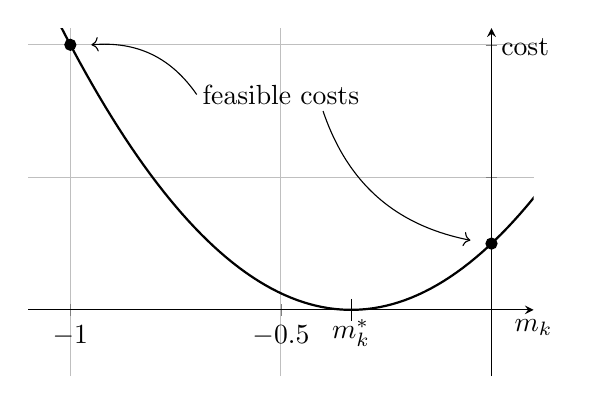
\begin{tikzpicture}
	\begin{axis}[axis lines=middle,
		xlabel={$m_k$}, xlabel style={below},
		ylabel={cost},
		xmin=-1.1, xmax=0.1, xtick={-1, -0.5, 0},
		ymin=-1, ymax=4.25, yticklabels={},
		grid=both,
		width=8cm,
		height=6cm]
		\addplot[domain=-1.25:0.25, samples=100, thick] {(1 + 3*x)^2};
		\addplot[only marks, mark=+, mark size=4pt] coordinates {(-1/3,0)};
		\node at (axis cs:-1/3,0) [anchor=north] {$m_k^*$};
		\addplot[only marks, mark=*] coordinates {(-1,4)};
		\addplot[only marks, mark=*] coordinates {(0,1)};
		\node at (axis cs:-0.5,3.25) {feasible costs};
		\draw[->, bend right=30] (axis cs:-0.7, 3.25) to (axis cs:-0.95,4);
		\draw[->, bend right=30] (axis cs:-0.4, 3) to (axis cs:-0.05,1.05);
	\end{axis}
\end{tikzpicture}
\end{center}

As we change the values of $M$ and $k$, the parabola shifts around, getting taller for larger $M$ and shifting leftward as $k \rightarrow M$.

We can see that for $k \in [0, \frac{M}{2})$, the $m_k = 0$ solution is lower down the cost curve, and for $k \in (\frac{M}{2}, M]$, the $m_k = -1$ solution is more optimal. ``If $k = \frac{M}{2}$ for even $M$), however, there is an ambiguity: either $m_k = 0$ or -1 gives the same value $(k + m_k M)^2 = (\frac{M}{2})^2$. For this $Y_{M/2}$ term (the ``Nyquist" term), we can arbitrarily split up the 

\printendnotes

\begin{thebibliography}{99} % https://tex.stackexchange.com/questions/198330/argument-in-thebibliography

\bibitem{lebesgue}
	Lebesgue Integrable, https://mathworld.wolfram.com/LebesgueIntegrable.html
\bibitem{hamming}
	Hamming, R., \textit{The Art of Doing Science and Engineering}
\bibitem{taylor}
	Simplest proof of Taylor's theorem, https://math.stackexchange.com/a/492165/278341
\bibitem{complex}
	Why do Fourier transforms use complex numbers?, https://math.stackexchange.com/a/1293127/278341
\bibitem{swarthmore}
	Derivation of Fourier Series, http://lpsa.swarthmore.edu/Fourier/Series/DerFS.html
\bibitem{medium}
	Nakagome, S. Fourier Transform 101 — Part 4: Discrete Fourier Transform, https://medium.com/sho-jp/fourier-transform-101-part-4-discrete-fourier-transform-8fc3fbb763f3
\bibitem{oppenheim}
	Oppenheim, A. \& Willsky, A., 1996, \textit{Signals and Systems, 2nd Ed.}
\bibitem{brunton}
	Brunton, S., The Fourier Transform and Derivatives, https://www.youtube.com/watch?v=d5d0ORQHNYs
\bibitem{kutz}
	\raggedright Kutz, J.N., 2023, \textit{Data-Driven Modeling \& Scientific Computation}, Ch. 11, https://faculty.washington.edu/kutz/kutz\_book\_v2.pdf
\bibitem{numpy}
	Discrete Fourier Transform, https://numpy.org/doc/2.1/reference/routines.fft.html
\bibitem{bristow}
	Bristow-Johnson, R., 2014, About Discrete Fourier Transform vs. Discrete Fourier Series, https://dsp.stackexchange.com/a/18931/40873
\bibitem{johnson}
	https://math.mit.edu/~stevenj/fft-deriv.pdf


\end{thebibliography}




\end{document}